\documentclass[tikz]{standalone}
\usetikzlibrary{decorations.markings}
\usetikzlibrary{arrows}
\begin{document}
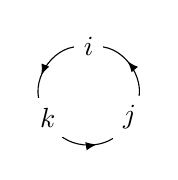
\begin{tikzpicture}
\def\rradiuS{.6}
%\draw (0,0) circle (\rradiuS cm);
\node (i) at (0,\rradiuS) {};
\node (j) at ({\rradiuS*cos(-30)},{\rradiuS* sin(-30)}) {};
\node (k) at (({\rradiuS*cos(210)},{\rradiuS* sin(210)}) {};
\path[draw,%
          decoration={%
            markings,%
            mark=at position 0.6   with \arrow{latex},%
          },%
          postaction=decorate] (j)  
          to[out=60, in=0] (i);
\path[draw,%
          decoration={%
            markings,%
            mark=at position 0.6   with \arrow{latex},%
          },%
          postaction=decorate] (i)
          to[out=180, in=120] (k);
\path[draw,%
          decoration={%
            markings,%
            mark=at position 0.6   with \arrow{latex},%
          },%
          postaction=decorate] (k) 
          to[out=-60, in=-120] (j);
\node[fill=white,draw=white] at (i) {\(i\)};
\node[fill=white,draw=white] at (j) {\(j\)};
\node[fill=white,draw=white] at (k) {\(k\)};
\end{tikzpicture}
\end{document}